\documentclass[12pt,a4paper]{article}
\input{stage1.sty}%
% Fichier de style stage2.sty [UTF8]
% Copyleft Laurent Bretonnière, laurent.bretonniere@gmail.com
% Version du 16/03/2015

\usepackage{mathtools}%	
\usepackage{fancybox}%
\usepackage{lastpage}%

\usepackage{fancyhdr}%
\renewcommand{\headrulewidth}{0.8pt}%
\renewcommand{\footrulewidth}{0.8pt}%

\usepackage[tikz]{bclogo}%
\renewcommand\bcStyleTitre[1]{\normalsize\textbf{#1}\smallskip}%
\renewcommand\logowidth{0pt}%

\newcommand{\fin}{\begin{center}%
$\clubsuit\clubsuit\clubsuit$%
\end{center}}%

\newcommand{\un}{\ding{192}\xspace}%
\newcommand{\deux}{\ding{193}\xspace}%
\newcommand{\trois}{\ding{194}\xspace}%
\newcommand{\quatre}{\ding{195}\xspace}%
\newcommand{\cinq}{\ding{196}\xspace}%
\newcommand{\six}{\ding{197}\xspace}%
\newcommand{\sept}{\ding{198}\xspace}%
\newcommand{\huit}{\ding{199}\xspace}%
\newcommand{\neuf}{\ding{200}\xspace}%

\setlength{\headheight}{15pt}%

%*********************************************************************************************
% Cours
%*********************************************************************************************

\usepackage[Lenny]{fncychap}%
\ChNumVar{\fontsize{76}{80}\usefont{OT1}{pzc}{m}{n}\selectfont}%
\ChTitleVar{\raggedleft\Huge\sffamily\bfseries}%

\renewcommand{\thesection}{\Roman{section})}%
\renewcommand{\thesubsection}{\arabic{subsection})}%
\renewcommand{\thesubsubsection}{\alph{subsubsection})}%

%*********************************************************************************************
% Environnements prédéfinis BCLOGO
%*********************************************************************************************

%% Lemme
\newenvironment{lem}{\begin{bclogo}[couleurBord=black!50,arrondi=0.1,logo=\hspace{17pt},barre=none]{Lemme :}}{\end{bclogo}\medskip}%

%% Propriété
\newenvironment{prop}[1][]{\begin{bclogo}[couleur=black!10,couleurBord=black!50,arrondi=0.1,logo=\hspace{17pt},barre=none]{Propriété :~#1}}{\end{bclogo}}%

%% Théorème
\newlength{\textlarg}
\settowidth{\textlarg}{~}
\newenvironment{theo}[1][\hspace{-\textlarg} :]{\begin{bclogo}[couleur=black!5,couleurBord=black!50,arrondi=0.1,logo=\hspace{17pt}, barre=none]{Théorème~#1}}{\end{bclogo}\medskip}%

\newenvironment{theon}[1][]{\begin{bclogo}[couleur=black!5,couleurBord=black!50,arrondi=0.1,logo=\hspace{17pt}, barre=none]{Théorème :~#1}}{\end{bclogo}\medskip}%

%% Corollaire
\newenvironment{coro}[1][]{\begin{bclogo}[couleurBord=black!50,arrondi=0.1,logo=\hspace{17pt},barre=none]{Corollaire :~#1}}{\end{bclogo}\medskip}%

%% Définition(s)

\newenvironment{defi}{\begin{bclogo}[couleur=black!10,couleurBord=black!50,arrondi=0.1,logo=\hspace{17pt}, barre=none]{Définition :}}{\end{bclogo}\medskip}%

\newenvironment{defis}{\begin{bclogo}[couleurBord=black!50,arrondi=0.1,logo=\hspace{17pt}, barre=none]{Définitions :}}{\end{bclogo}\medskip}%

%% Preuve
\newenvironment{pf}{\renewcommand\logowidth{17pt}\begin{bclogo}[noborder=true,logo=\hspace{17pt},couleurBarre=black!25,epBarre=3.5]{Démonstration :}}{\hspace*{\fill}$\Box$\end{bclogo}\smallskip\renewcommand\logowidth{0pt}}%

%\blacksquare

%% Notation
\newenvironment{nota}{\begin{bclogo}[couleurBord=black!50,arrondi=0.1,logo=\hspace{17pt},barre=none]{Notation :}}{\medskip}%

%% Exercice et Exercice-type
\newenvironment{exo}{$\circledast$ \quad\textsc{\underline{exercice} :}~}{\hspace*{\fill}$\circledast$\vskip 8pt}
\newenvironment{type}{$\blacktriangleright$ \quad\textsc{exercice-type :}~}{\hspace*{\fill}$\blacktriangleleft$\vskip 8pt}

%% Exemple(s)
\newenvironment{exem}{\textbf{Exemple :}~}{\medskip}
\newenvironment{exems}{\textbf{Exemples :}~}{\medskip}

%% Remarque(s)
\newenvironment{rem}{\textbf{Remarque :}~}{\medskip}
\newenvironment{rems}{\textbf{Remarques :}~}{\medskip}

%% Rappel(s)
\newenvironment{rap}{\textbf{Rappel :}~}{\medskip}
\newenvironment{raps}{\textbf{Rappels :}~}{\medskip}

%% Cas particulier(s)
\newenvironment{cp}{\textbf{Cas particulier :}~}{\medskip}
\newenvironment{cps}{\textbf{Cas particuliers :}~}{\medskip}

%% Application
\newenvironment{appli}{\textbf{Application :}~}{\medskip}%{\medskip} %
\usepackage[left=1.5cm,right=1.5cm,top=1cm,bottom=1cm]{geometry}
\usepackage{pst-plot,pst-text,pstricks,pst-tree,pstricks-add}
\usepackage{tabularx}
\usepackage{graphicx}



\begin{document}

\pagestyle{empty}
\begin{center}{\LARGE \textbf{\textsc{DS affines-corrigé}}}\end{center}

\textbf{\textsc{\underline{Exercice 1:}}}
\begin{enumerate}
\item \medskip 
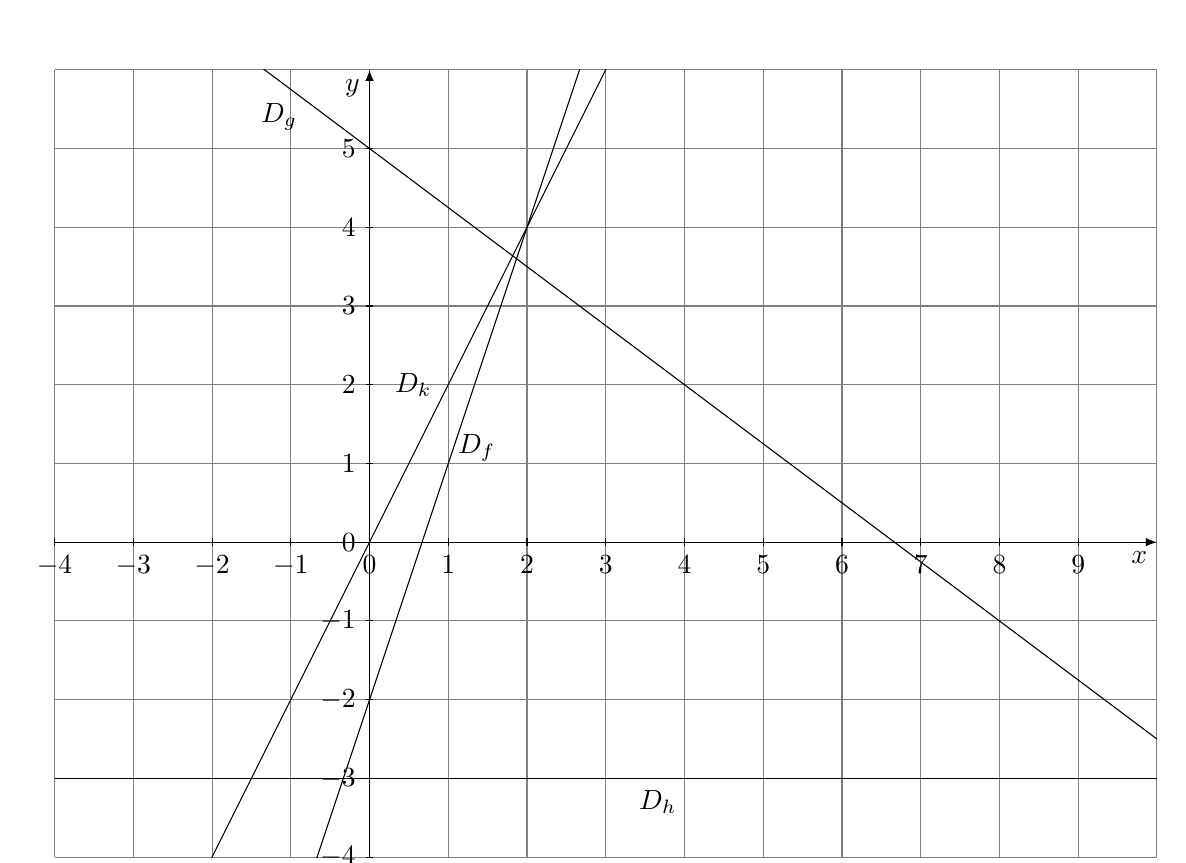
\begin{tikzpicture}[x=10mm,y=10mm]
\draw [gray,xstep=1,ystep=1] (-4,-4) grid (10,6);
\draw [->,>=latex] (-4,0) -- (10,0) node [below left] {$x$};
\draw [->,>=latex] (0,-4) -- (0,6) node [below left] {$y$};

\foreach \x in {-4,...,9}
\draw (\x,0.5mm) -- (\x,-0.5mm) node [below] {$\x$};
\foreach \y in {-4,...,5}
\draw (0.5mm,\y) -- (-0.5mm,\y) node [left] {$\y$};

%\draw (0,0) node [below left] {$O$};

\clip (-4,-4) rectangle (10,6);
\draw [domain=-4:10,samples=100] plot (\x,{3*\x-2});
\draw [domain=-4:10,samples=100] plot (\x,{2*\x});
\draw [domain=-4:10,samples=100] plot (\x,{-(3/4)*\x+5});
\draw [domain=-4:10,samples=100] plot (\x,{-3});
\draw (-1.5,5.4) node [right] {$\mathscr{D}_{g}$};
\draw (1,1.2) node [right] {$\mathscr{D}_{f}$};
\draw (0.2,2) node [right] {$\mathscr{D}_{k}$};
\draw (3.3,-3.3) node [right] {$\mathscr{D}_{h}$};
\end{tikzpicture}
\medskip
\item $f_{1}(x)=-\frac{1}{3} x+4$\hfill $f_{2}(x)=\frac{3}{4}x-2$\hfill $f_{3}(x)=4$\hfill $f_{4}(x)=-x$
\end{enumerate}

\vspace{0,5cm}

\textbf{\textsc{\underline{Exercice 2:}}}\\
coefficient directeur: $m=\frac{f(5)-f(-2)}{5-(-2)}=\frac{7-4}{5-(-2)}=\frac{3}{7}$ (différence des ordonnées divisée par celle des abscisses).\\
donc $f(x)=\frac{3}{7}x+p$ (avec $p\in\R$).\\
Or $f(-2)=4$ donc $\frac{3}{7}\x (-2)+p=4$ donc $-\frac{6}{7}+p=4$ donc $p=4+\frac{6}{7}=\frac{34}{7}$.\\
Finalement: $f(x)=\frac{3}{7}x+\frac{34}{7}$

\vspace{0,5cm}

\textbf{\textsc{\underline{Exercice 3:}}}
\begin{enumerate}
\item $f(x)=g(x)\iff 5x-2=\frac{5}{3}x+6\iff 5x-\frac{5}{3}x=6+2\iff \frac{15}{3}x-\frac{5}{3}x=8$\medskip\\
$\iff \frac{10}{3}x=8\iff x=\frac{8}{\frac{10}{3}}=8\x \frac{3}{10}=\frac{12}{5}$.\medskip\\
Donc le point cherché a pour coordonnées $(\frac{12}{5};10)$.
\item $f(2)=5\x2-2=8\neq 7$ donc le point de coordonnées $(2;7)$ ne se trouve pas sur la courbe de $f$.\medskip 
\end{enumerate}

\vspace{0,5cm}

\textbf{\textsc{\underline{Exercice 4:}}}\medskip
\begin{enumerate}
\item 
Valeurs d'annulation: $2x-4=0\iff 2x=4\iff x=\frac{4}{2}=2$\\
$-3x-5=0\iff -3x=5\iff x=\frac{5}{-3}=-\frac{5}{3}$
\begin{center}
\begin{tikzpicture}
			\tkzTabInit[lgt=4,espcl=2]%
			{$x$/1, $2x-4$/0.8, $-3x-5$/0.8, $(2x-4)(-3x-5)$/0.8}%
			{$-\infty$,$-\frac{5}{3}$, $2$,$+\infty$}%
			\tkzTabLine{ , - , t , - , z, +,}
			\tkzTabLine{ , + , z , - , t, -,}
			\tkzTabLine{ , - , z , + , z, -,}
\end{tikzpicture}
\end{center}
\medskip
\item Valeur d'annulation: $-3x+9=0\iff -3x=-9\iff x=\frac{-9}{-3}=3$\\
valeur INTERDITE (sinon division par zéro): $7x-5=0\iff 7x=5\iff x=\frac{5}{7}$
\begin{center}
\begin{tikzpicture}
			\tkzTabInit[lgt=4,espcl=2]%
			{$x$/1, $-3x-9$/0.8, $7x-5$/0.8, $\frac{-3x+9}{7x-5}$/1}%
			{$-\infty$,$\frac{5}{7}$, $3$,$+\infty$}%
			\tkzTabLine{ , + , t , + , z, -,}
			\tkzTabLine{ , - , z , + , t, +,}
			\tkzTabLine{ , - , d , + , z, -,}
\end{tikzpicture}
\end{center}
\item $S=]-\infty;-\frac{5}{3}[\cup ]2;+\infty[$ (on donne les zones où il y a $-$ car $<0$ signifie $-$; crochets ouverts car "strictement")\medskip
\item $S=]-\frac{5}{3};3]$ ($\geqslant 0$ signifie $+$ (y compris 0), et on "rejette" la valeur interdite d'où crochet ouvert pour elle)
\end{enumerate}
\vspace{0,5cm}
\textbf{\textsc{\underline{Exercice 5:}}}\medskip\\
$f$ n'est pas affine car c'est une fonction du second degré (ou: $f(x)$ n'est pas de la forme $mx+p$).\medskip\\
$g(x)=\frac{3x-5}{7}=\frac{3}{7}x-\frac{5}{7}$. $g$ est affine de coefficient directeur $\frac{3}{7}$ car $g(x)$ est de la forme $mx+p$ avec $m=\frac{3}{7}$.\\
$h(x)=(x-3)(2x-5)-2x^2=2x^2-5x-6x+15-2x^2=-11x+15$\medskip\\
$h(x)=mx+p$ avec $m=-11$ donc $h$ est affine de coefficient directeur $-11$.


\end{document}